\chapter{Monitoring a Hadoop Cluster}\label{chap:6}
In this chapter, we will cover:
\begin{itemize}
  \item Monitoring Hadoop cluster with JMX
  \item Monitoring Hadoop cluster with Ganglia
  \item Monitoring Hadoop cluster with Nagios
  \item Monitoring Hadoop cluster with Ambari
  \item Monitoring Hadoop cluster with Chukwa
\end{itemize}

\section{Introduction}
System monitoring is critical for maintaining the health and availability for large distributed systems such as Hadoop. General monitoring tasks include monitoring the health of cluster nodes and networks, such as the usage of memory, heap, CPU and network etc. For a Hadoop cluster, we may also want to monitor some specific metrics such as the status of jobs and tasks in the cluster, the status of the JobTracker, TaskTracker, NameNode and DataNode and so on.

Hadoop is lucky to be born in an open source world! A number of very stable open source tools for system monitoring are there waiting to join the Hadoop family. And many of these systems have been adopted by Hadoop for monitoring purposes.

In this chapter, we will first introduce the management framework Java Management Extension (JMX) for system monitoring. Next, we will introduce two famous open source cluster monitoring systems: Ganglia and Nagios. Ganglia is an open source scalable monitoring system. Monitoring daemons running on monitoring hosts send data to monitoring server hosts for storage, statistical analysis and visualization. Nagios is another famous monitoring system. It monitors hosts in the cluster using plugins.

Next, we will introduce Hadoop specific monitoring systems Ambari and Chukwa. Ambari was designed to be a full-fledged system for the deployment, management and monitoring of Hadoop clusters. It was developed based on the monitoring framework of Ganglia and Nagios. But different from Ganglia and Nagios, Apache Chukwa monitors a Hadoop cluster by analysing system logs collected from the Hadoop cluster. Apache Flume is another general purpose data analytics framework for streaming data such as system logs. It can be configured to do system monitoring, which is similar to Chukwa.

\section{Monitoring Hadoop cluster with JMX}
Java Management eXtensions (JMX) is the technology used by Java to build, monitor and manage distributed systems and network applications. It has been incorporated into Java since J2SE platform 5.0. For more information about JMX, please visit the official website at \url{http://www.oracle.com/technetwork/java/javase/tech/javamanagement-140525.html}. In this recipe, we will outline steps to configure Hadoop cluster monitoring with JMX.
\begin{info}
Notice: \\
In this chapter, we assume to monitor Hadoop version 1.1.y or the corresponding 0.20.x Hadoop release. Configurations for monitoring Hadoop versions 2.0.x or 0.23.x should follow the recipe with some changes.
\end{info}

\subsection*{Getting ready}
We assume that Oracle JDK has been installed and our Hadoop cluster has been configured properly and all the daemons are running without any problems.

\subsection*{How to do it...}
 Use the following recipe to configure JMX for monitoring a Hadoop cluster:

Create a JMX password file for remote monitoring with command:
\lstset{style=bashstyle}
\begin{lstlisting}[language=bash]
$ cp $JAVA_HOME/jre/lib/management/jmxremote.password.template $HADOOP_HOME/conf/jmxremote.password
\end{lstlisting}

Open the template password file \verb|$HADOOP_HOME/conf/jmxremote.password| with a text editor and the last a few lines of this file will be similar to the following: 
\lstset{style=bashstyle}
\begin{lstlisting}
# Following are two commented-out entries.  The "measureRole" role has
# password "QED".  The "controlRole" role has password "R&D".
#
# monitorRole  QED
# controlRole  R&D
Remove the comment symbol ``#" for the two highlighted lines.
\end{lstlisting}

These two lines specify the passwords for monitorRole and controlRole. JMX will use them for authentication purposes in a remote monitoring.

Change the permission of the password file to 600 with command: \\
\verb|$ chmod 600 $HADOOP_HOME/conf/jmxremote.password|
\begin{warning}
Warning! \\
If this file is too open, you will get error similar to the following when starting the Hadoop cluster daemons:
\lstset{style=bashstyle}
\begin{lstlisting}
master: Error: Password file read access must be restricted: /usr/local/hadoop/conf/jmxremote.password
\end{lstlisting}
\end{warning}

Open file \verb|$HADOOP_HOME/conf/hadoop-env.sh| with a text editor.

In this file, we will be able to find JMX monitoring configurations for the Hadoop daemons including \emph{NameNode, SecondaryNameNode, DataNode, balancer, JobTracker} and \emph{TaskTracker}. The default configuration will be similar to the following:
\lstset{style=bashstyle}
\begin{lstlisting}
export HADOOP_NAMENODE_OPTS="-Dcom.sun.management.jmxremote $HADOOP_NAMENODE_OPTS"
export HADOOP_SECONDARYNAMENODE_OPTS="-Dcom.sun.management.jmxremote $HADOOP_SECONDARYNAMENODE_OPTS"
export HADOOP_DATANODE_OPTS="-Dcom.sun.management.jmxremote $HADOOP_DATANODE_OPTS"
export HADOOP_BALANCER_OPTS="-Dcom.sun.management.jmxremote $HADOOP_BALANCER_OPTS"
export HADOOP_JOBTRACKER_OPTS="-Dcom.sun.management.jmxremote $HADOOP_JOBTRACKER_OPTS"
\end{lstlisting}

Now, we need to configure remote monitoring port for Hadoop daemons by changing the original configuration to the following: 
\lstset{style=bashstyle}
\begin{lstlisting}
# Extra Java runtime options. Empty by default.
export HADOOP_OPTS="-Dcom.sun.management.jmxremote.authenticate=true -Dcom.sun.management.jmxremote.ssl=false -Dcom.sun.management.jmxremote.password.file=$HADOOP_CONF_DIR/jmxremote.password"

export HADOOP_NAMENODE_OPTS="-Dcom.sun.management.jmxremote $HADOOP_NAMENODE_OPTS -Dcom.sun.management.jmxremote.port=8004"
export HADOOP_SECONDARYNAMENODE_OPTS="-Dcom.sun.management.jmxremote $HADOOP_SECONDARYNAMENODE_OPTS -Dcom.sun.management.jmxremote.port=8005"
export HADOOP_DATANODE_OPTS="-Dcom.sun.management.jmxremote $HADOOP_DATANODE_OPTS -Dcom.sun.management.jmxremote.port=8006"
export HADOOP_BALANCER_OPTS="-Dcom.sun.management.jmxremote $HADOOP_BALANCER_OPTS -Dcom.sun.management.jmxremote.port=8007"
export HADOOP_JOBTRACKER_OPTS="-Dcom.sun.management.jmxremote $HADOOP_JOBTRACKER_OPTS -Dcom.sun.management.jmxremote.port=8008"
export HADOOP_TASKTRACKER_OPTS="-Dcom.sun.management.jmxremote.port=8009"
\end{lstlisting}


Use the following command to start the monitor user interface: \\
\verb|$ jconsole| \\

We can see a window that is similar to Figure \ref{fig:jconsole}.
\begin{figure}[ht]
  \centering
  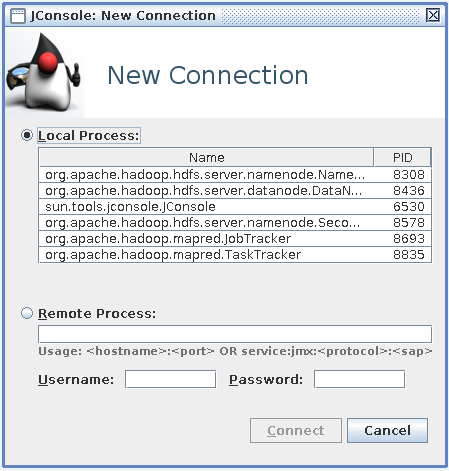
\includegraphics[width=.7\textwidth]{figs/5163os_06_01.png}
  \caption{jconsole UI}\label{fig:jconsole}
\end{figure} 
From this window, we can check the status of both local and remote processes. Checking the status of local processes is relatively simple. First, select the desired process to check from the process list. Then, we only need to click the ``Connect'' button. Checking the status of remote processes is relatively complicated. We need to specify the location of the service by either specifying hostname and port or protocol and sap as shown in Figure \ref{fig:jconsole}. We also need to enter the username and password for authentication purposes.  In the following steps, we assume to check the status of local JobTracker process.

Select the ``Local Process'' radio button and then click ``Connect'' button. We can get a monitoring window, as shown in Figure \ref{fig:jconsole.jobtracker} after waiting for a few moments.
\begin{figure}[ht]
  \centering
  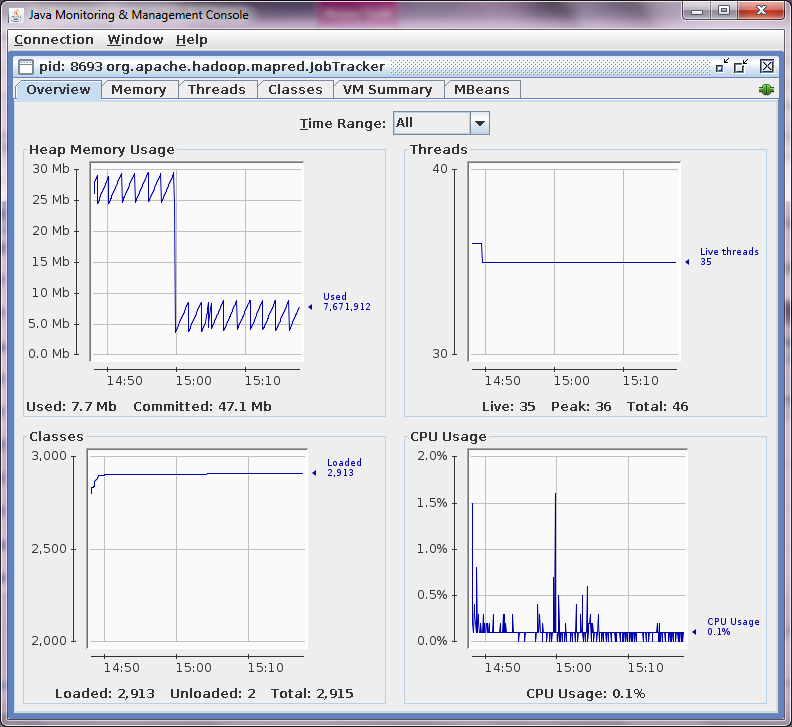
\includegraphics[width=.7\textwidth]{figs/5163os_06_02.png}
  \caption{jconsole JobTracker resource usage monitoring UI}\label{fig:jconsole.jobtracker}
\end{figure} 
The window shows the daemon status for the JobTracker. From the window, we can check the memory usage, threads, classes, summary of JVM and details of MBeans.

Check the memory of the daemon by clicking on the "Memory" tab of the jconsole window and we will get a window similar to Figure \ref{fig:heap.usage.window}.
\begin{figure}[ht]
  \centering
  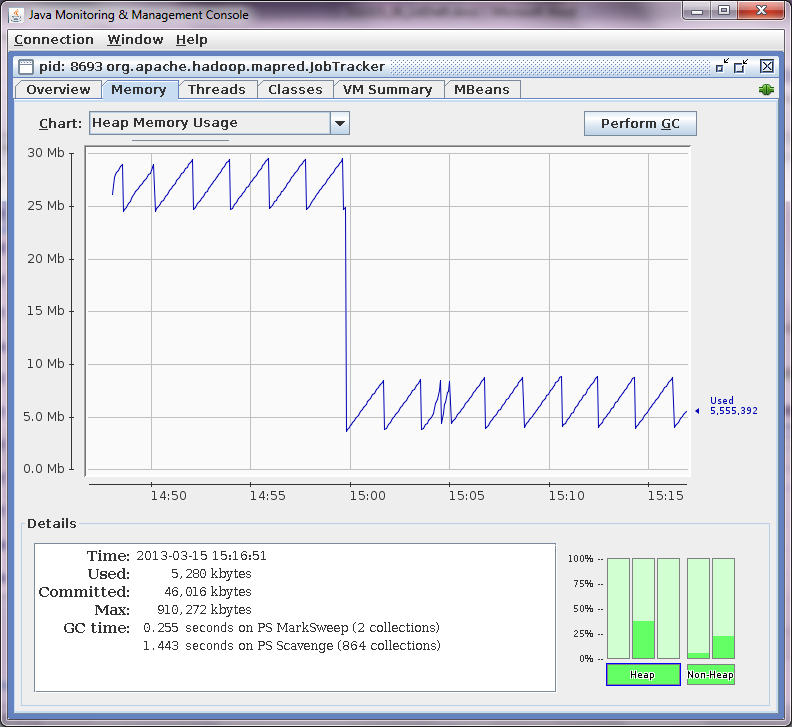
\includegraphics[width=.7\textwidth]{figs/5163os_06_03.png}
  \caption{The Heap Memory Usage Window}\label{fig:heap.usage.window}
\end{figure} 
The memory window shows the heap memory usage as a time serial chart. From this window, we can select from different charts and time ranges to display. The bottom part of the window is a summary of the current memory usage.

By clicking on the "Threads" tab of the window, we can check the running threads of the JobTracker and we can get a window similar to Figure \ref{fig:num.threads}.
\begin{figure}[ht]
  \centering
  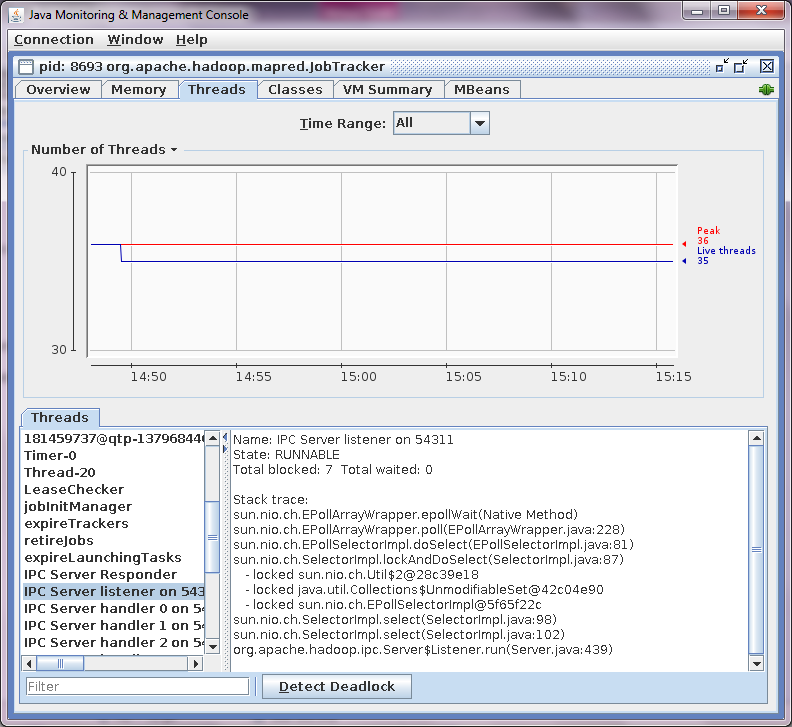
\includegraphics[width=.7\textwidth]{figs/5163os_06_04.png}
  \caption{Number of Threads Window}\label{fig:num.threads}
\end{figure} 
The upper part of the window shows the number of peak live threads and the number of current live threads. On the lower part of the window, we can see a list of threads, the information of which can be viewed by clicking on the desired thread names.
Similarly, we can check the current classes by clicking on the "Classes" tab of the window and check the summary of the JVM virtual machine by clicking on the "VM Summary" tab of the window.

The "MBeans" tab is the most informative one if you want to check the status details of the daemon. For example, Figure \ref{fig:mbeans.hadoop.metrics} shows more metrics details for JobTracker:
\begin{figure}[ht]
  \centering
  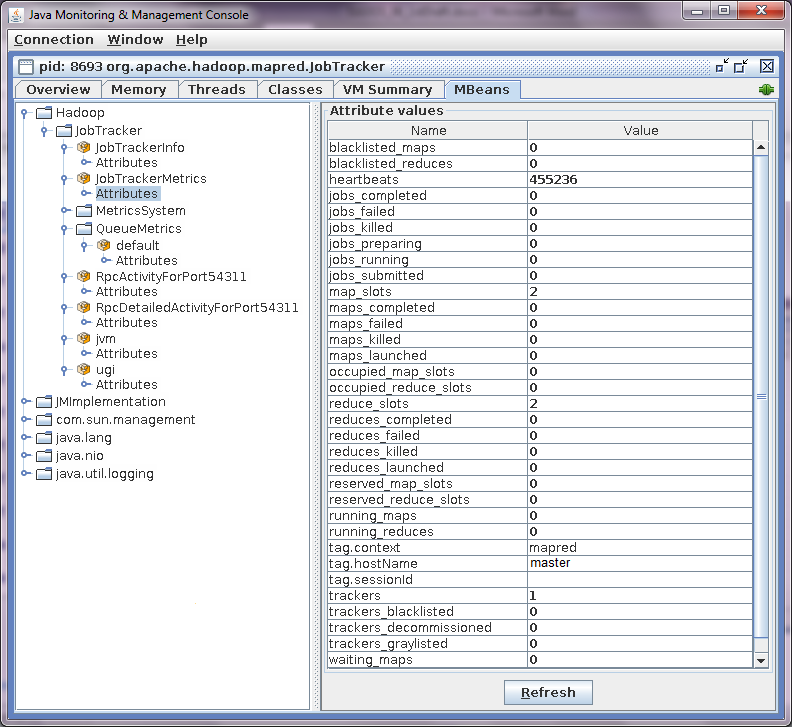
\includegraphics[width=.7\textwidth]{figs/5163os_06_05.png}
  \caption{MBeans Hadoop Metrics}\label{fig:mbeans.hadoop.metrics}
\end{figure} 
From this window, we can get a number of JobTracker metrics such as number of running jobs, number of map and reduce slots and number of running map and reduce tasks etc.
\subsection*{See also}
\begin{itemize}
  \item Monitoring Hadoop cluster with Ganglia
  \item Monitoring Hadoop cluster with Nagios
  \item Monitoring Hadoop cluster with Ambari
  \item Monitoring Hadoop cluster with Chukwa
  \item \url{http://docs.oracle.com/javase/tutorial/jmx/}
  \item \url{docs.oracle.com/javase/tutorial/jmx/}
\end{itemize}

\section{Monitoring Hadoop cluster with Ganglia}
Ganglia is an open source, scalable and distributed monitoring system for clusters and computing grids. It has three major components: the monitoring daemon, the metadata daemon and the web UI. In this recipe, we will outline steps to configure Ganglia for Hadoop cluster monitoring.
\subsection*{Getting ready}
Login to the master node from administrator machine with command: \\
\verb|$ ssh hdadmin@master| \\

Use the following yum command to install Ganglia on the master machine: 
\lstset{style=bashstyle}
\begin{lstlisting}[language=bash]
$ sudo yum install -y ganglia-gmond ganglia-gmetad ganglia-web
\end{lstlisting}

Install Ganglia monitoring daemon on all the slave nodes with command:
\lstset{style=bashstyle}
\begin{lstlisting}[language=bash]
for host in `cat $HADOOP_HOME/conf/slaves`
do
  echo "Installing Ganglia on host " $host
  sudo ssh $host -C "yum install -y ganglia-gmond"
done
\end{lstlisting}

In this recipe, we assume that the Ganglia server will run on the master node and the monitoring daemons run on both master and slave nodes.
\subsection*{How to do it...}
 Use the following recipe to configure Ganglia for Hadoop cluster monitoring:

Open the gmond configuration file \verb|/etc/ganglia/gmond.conf| with a text editor.

Change the cluster attribute to:
\lstset{style=bashstyle}
\begin{lstlisting}
cluster {
  name = "hadoop"
  owner = "hduser"
  latlong = "unspecified"
  url = "unspecified"
}
\end{lstlisting}

Change the \verb|udp_send_channel| attribute to: 
\lstset{style=bashstyle}
\begin{lstlisting}
udp_send_channel {
  bind_hostname = yes
  # mcast_join = 239.2.11.71
  host = master
  port = 8649
  ttl = 1
}
\end{lstlisting}

Change the \verb|udp_recv_channel| attribute to: 
\lstset{style=bashstyle}
\begin{lstlisting}
udp_recv_channel {
  # mcast_join = 239.2.11.71
  port = 8649
  # bind = 239.2.11.71
}
\end{lstlisting}

Hadoop supports network communication through both unicast (with normal IP addresses, which is the one we use here) and multicast, which uses multicast address such as \emph{239.2.11.71}. To use multicast, all the monitored hosts should be in the same IP segment. In this book, we assume to use unicast.

Add all the hostnames in the cluster to the gmetad configuration file /etc/ganglia/gmetad.conf, for example, this file should contain the following: \\
\verb|data_source "hdcluster" master:8649|

Here "\textbf{hdcluster}" is the name of cluster that Ganglia monitors and "\textbf{master:8649}" is the network address of gmetad.

Open file \verb|$HADOOP_HOME/conf/hadoop-metrics.properties| with your favorite text editor and add the following contents into the file:
\lstset{style=bashstyle}
\begin{lstlisting}
jvm.class=org.apache.hadoop.metrics.ganglia.GangliaContext
jvm.period=10
jvm.servers=master:8649
rpc.class=org.apache.hadoop.metrics.ganglia.GangliaContext
rpc.period=10
rpc.servers=master:8649
dfs.class=org.apache.hadoop.metrics.ganglia.GangliaContext
dfs.period=10
dfs.servers=master:8649
mapred.class=org.apache.hadoop.metrics.ganglia.GangliaContext
mapred.period=10
mapred.servers=master:8649
hbase.class=org.apache.hadoop.metrics.ganglia.GangliaContext
hbase.period=10
hbase.servers=master:8649
\end{lstlisting}

In the above configuration, we have specified three common parameters: class, period and servers. Parameter class specifies the message format that Ganglia will use (can be either GangliaContext or GangliaContext31); period specifies the time interval between two consecutive metric updates and servers specifies a list of server that monitoring messages should be sent to.

Copy configuration files to all the slave nodes with command: 
\lstset{style=bashstyle}
\begin{lstlisting}[language=bash]
for host in `cat $HADOOP_HOME/conf/slaves`
do
  echo "Copying ganglia monitoring configuration file to host" $host;
  sudo scp /etc/ganglia/gmond.conf $host:/etc/ganglia/gmond.conf
  sudo scp /etc/ganglia/gmetad.conf $host:/etc/ganglia/gmetad.conf
  sudo scp $HADOOP_HOME/conf/hadoop-metrics.properties $host:$HADOOP_HOME/conf/hadoop-metrics.properties;
done
\end{lstlisting}

Restart the Hadoop cluster with commands:
\lstset{style=bashstyle}
\begin{lstlisting}[language=bash]
$ stop-all.sh
$ start-all.sh
\end{lstlisting}

Start gmond daemon with command on the master node: \\
\verb|$ sudo service gmond start|

Run command: \verb|$ sudo chkconfig gmond on| if you want the process to survive a system reboot.

Check the status of gmond with command: 
\lstset{style=bashstyle}
\begin{lstlisting}[language=XML]
$ curl master:8649
<GANGLIA_XML VERSION="3.1.7" SOURCE="gmond">
<CLUSTER NAME="hdcluster" LOCALTIME="1363403519" OWNER="hduser" LATLONG="unspecified" URL="hdcluster.com">
<HOST NAME="master" IP="10.147.166.55" REPORTED="1363403500" TN="19" TMAX="20" DMAX="0" LOCATION="unspecified" GMOND_STARTED="1363403380">
<METRIC NAME="proc_run" VAL="3" TYPE="uint32" UNITS=" " TN="42" TMAX="950" DMAX="0" SLOPE="both">
<EXTRA_DATA>
<EXTRA_ELEMENT NAME="GROUP" VAL="process"/>
<EXTRA_ELEMENT NAME="DESC" VAL="Total number of running processes"/>
<EXTRA_ELEMENT NAME="TITLE" VAL="Total Running Processes"/>
</EXTRA_DATA>
</METRIC>
<METRIC NAME="dfs.datanode.heartBeats_avg_time" VAL="1.0" TYPE="double" UNITS="" TN="2" TMAX="60" DMAX="0" SLOPE="both">
<EXTRA_DATA>
<EXTRA_ELEMENT NAME="GROUP" VAL="dfs.datanode"/>
</EXTRA_DATA>
</METRIC>
<METRIC NAME="mapred.shuffleOutput.shuffle_output_bytes" VAL="0" TYPE="float" UNITS="" TN="1225" TMAX="60" DMAX="0" SLOPE="positive">
<EXTRA_DATA>
<EXTRA_ELEMENT NAME="GROUP" VAL="mapred.shuffleOutput"/>
</EXTRA_DATA>
</METRIC>
...
<EXTRA_ELEMENT NAME="GROUP" VAL="system"/>
<EXTRA_ELEMENT NAME="DESC" VAL="Operating system release date"/>
<EXTRA_ELEMENT NAME="TITLE" VAL="Operating System Release"/>
</EXTRA_DATA>
</METRIC>
</HOST>
</CLUSTER>
</GANGLIA_XML>
\end{lstlisting}

The highlighted lines show that some HDFS and MapReduce metrics is being monitored by Ganglia.

Start gmetad daemon with command on the master node: \\
\verb|$ sudo service gmetad start|

Start gmond on all slave nodes with command: 
\lstset{style=bashstyle}
\begin{lstlisting}[language=bash]
for host in `cat $HADOOP_HOME/conf/slaves`
do
  echo "Starting gmond service on host: " $host;
  sudo ssh $host -C "service gmond start";
done
\end{lstlisting}

Open file \verb|/etc/httpd/conf.d/ganglia.conf| with your favorite text editor and add the following content: 
\lstset{style=bashstyle}
\begin{lstlisting}[language=XML]
<Location /ganglia>
   Order deny,allow
   Allow from all
</Location>
\end{lstlisting}

The access control setting in this file allows everyone to visit the Ganglia web UI. For security reasons, we can restrict the IP addresses, hosts or domains with the "Allow from" and "Deny from" statements in the configuration.

Start the httpd daemon with command: \\
\verb|$ sudo service httpd start|

Check the status of Ganglia by opening URL \url{http://master:80/ganglia} and we can get webpage similar to Figure \ref{fig:ganglia.cluster.summary}.
\begin{figure}[ht]
  \centering
  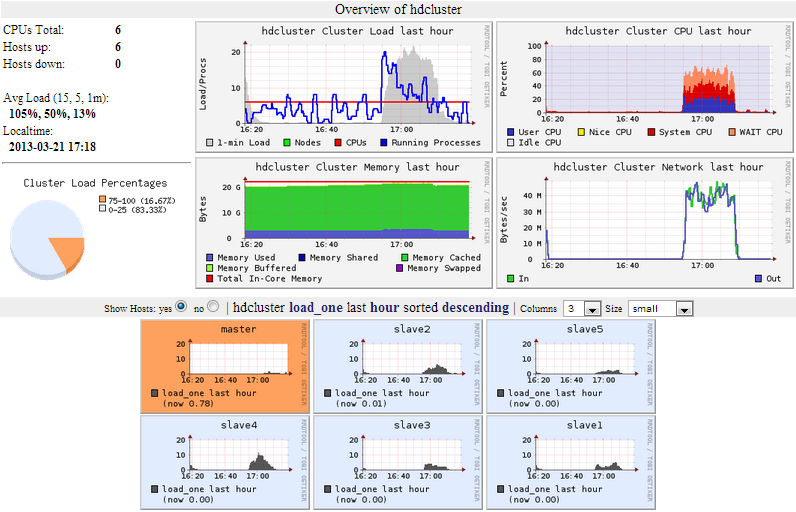
\includegraphics[width=.90\textwidth]{figs/5163os_06_06.png}
  \caption{Ganglia Cluster Summary}\label{fig:ganglia.cluster.summary}
\end{figure} 
The upper left portion of the UI is a summary of the cluster, including number of hosts, host status, average load etc.

The upper right part of Figure \ref{fig:ganglia.cluster.summary} shows an overview of the whole cluster, including cluster total load, cpu usage, memory and network traffic. It contains a clear jump for about 20 minutes when one teragen job is running, which consumes cluster resources.

The lower part of Figure \ref{fig:ganglia.cluster.summary} shows the status for each node in the cluster, including the master node and all the slave nodes. We can change the metric to display by selecting from the combo box as shown in Figure \ref{fig:ganglia.metrics}.
\begin{figure}[ht]
  \centering
  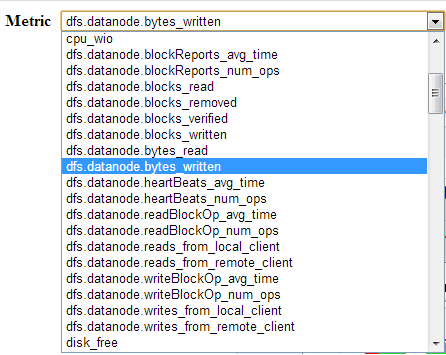
\includegraphics[width=.9\textwidth]{figs/5163os_06_09.png}
  \caption{Ganglia Available Monitoring Metrics}\label{fig:ganglia.metrics}
\end{figure} 
For example, by selecting metric "\verb|dfs_datenode.bytes_written|", we can get the \verb|bytes_written| for each node as shown in Figure \ref{fig:bytes.written.metric}.
\begin{figure}[ht]
  \centering
  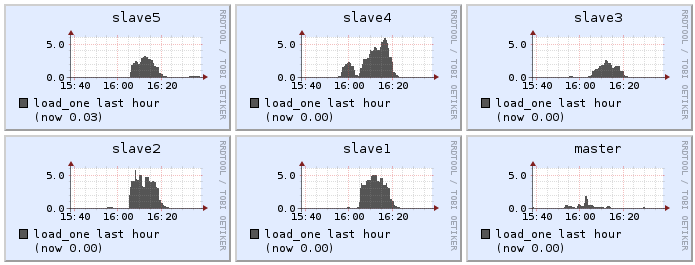
\includegraphics[width=.9\textwidth]{figs/5163os_06_10.png}
  \caption{The bytes written metric for all the Datanodes}\label{fig:bytes.written.metric}
\end{figure} 
 Figure \ref{fig:bytes.written.metric} confirms that a DataNode is the actual place where data blocks are stored and NameNode only keeps track of the metadata for the data blocks. So the written data size is much smaller for NameNode.

Check the details of each cluster node by selecting from the combo box, which has initial value of "--Choose a Node". For example, if we want to check all the metric for the master node, we will be able to get web page similar to Figure \ref{fig:master.status}.
\begin{figure}[ht]
  \centering
  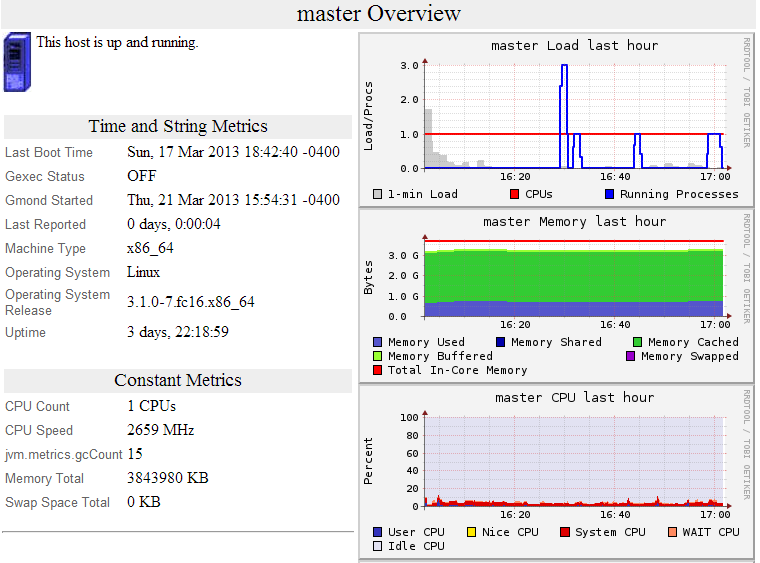
\includegraphics[width=.8\textwidth]{figs/5163os_06_11.png}
  \caption{Metric Status of the \textbf{master} Node}\label{fig:master.status}
\end{figure} 
By scrolling down the window, we can check the Hadoop JobTracker metrics as shown in Figure \ref{fig:jobtracker.metrics}.
\begin{figure}[ht]
  \centering
  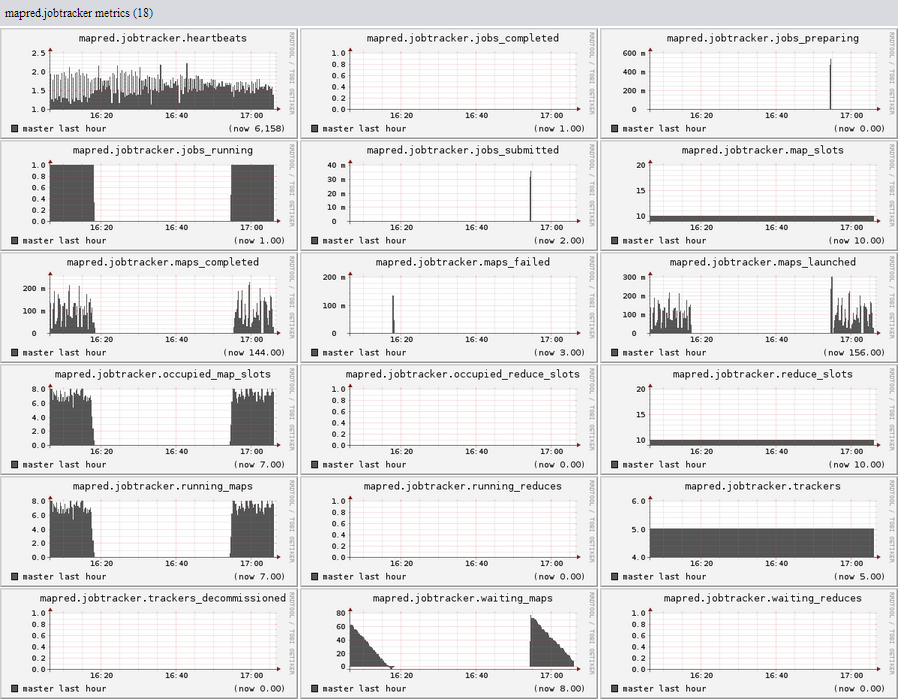
\includegraphics[width=.8\textwidth]{figs/5163os_06_12.png}
  \caption{MapReduce jobtracker metrics}\label{fig:jobtracker.metrics}
\end{figure} 
This screenshot contains the status information of the JobTracker including the number of running jobs, the number of map and reduce slots and so on.

\subsection*{How it works}
A Ganglia monitoring system is composed of three parts: the monitoring daemons gmond, the meta-data handling daemon gmetad and the web UI.

Ganglia gmond daemons run on each node that is being monitored in the cluster. They continuously collect metrics data and send to the gmetad daemon running on the master node. The gmetad daemon stores data into a database maintained by rrdtool. The web UI, including all the graphs, is generated with PHP by pulling the data from the database. The Ganglia data flow can be described with the following figure:
\begin{figure}[ht]
  \centering
  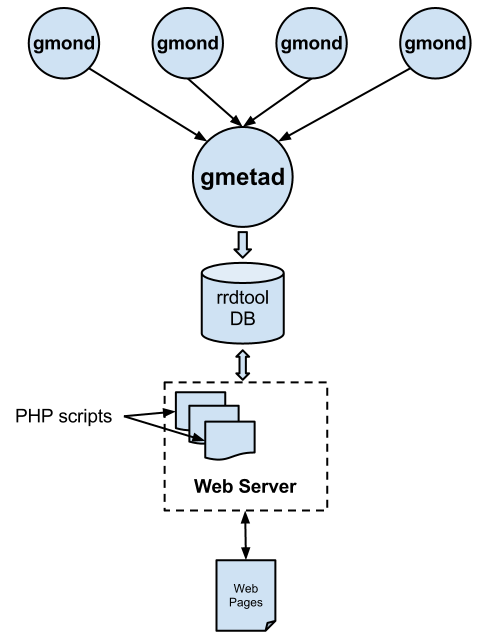
\includegraphics[width=.6\textwidth]{figs/5163os_06_13.png}
  \caption{The Ganglia Data Flow Diagram}\label{fig:ganglia.dataflow}
\end{figure} 
\subsection*{See also}
\begin{itemize}
  \item Monitoring Hadoop cluster with JMX
  \item Monitoring Hadoop cluster with Chukwa
  \item Monitoring Hadoop cluster with Nagios
  \item Monitoring Hadoop cluster with Ambari
  \item \url{http://ganglia.sourceforge.net/}
  \item \url{http://www.ibm.com/developerworks/wikis/display/WikiPtype/ganglia}
\end{itemize}
\section{Monitoring Hadoop cluster with Nagios}
Nagios is a powerful open source cluster monitoring system. It can monitor not only hosts and servers but also interconnecting devices such as routers and switches. The alerting services provide notification mechanism for fast response on system problems.

Designed to be a generic monitoring system, Nagios can be configured to monitor Hadoop clusters. In this recipe, we will outline steps to configure Nagios for Hadoop cluster monitoring.
\subsection*{Getting ready}
To get started with Nagios monitoring, we need to install it first. On CentOS and other Red Hat compatible Linux systems, we can use the following yum command to install Nagios:

\verb|$ sudo yum install nagios nagios-plugins|

This command will automatically install the dependency software packages such aslibgd and libgd-devel etc. After installation, the Nagios configuration files will be under directory /etc/nagios and the Nagios daemon will be under directory \verb|/etc/init.d/|.

Install Nagios Remote Plugin Executor (NRPE) package with command:\\
\verb|$ sudo yum install nrpe|

\emph{NRPE} is a Nagios add-on that allows us to execute Nagios plug-ins on a remote machine. For more information, please check: \url{http://nagios.sourceforge.net/docs/3_0/addons.html} and \url{http://nagios.sourceforge.net/docs/nrpe/NRPE.pdf}.

Download \verb|check_jmx| Nagios plugin from \url{http://exchange.nagios.org/directory/Plugins/Java-Applications-and-Servers/check_jmx/details}.

We want to use Java JMX\index{JMX} as a Nagios plugin to monitor Hadoop metrics.

Use the following commands to build the \verb|check_jmx| package:
\lstset{style=bashstyle}
\begin{lstlisting}[language=bash]
$ tar xvf check_jmx.tgz
$ cd check_jmx
$ ant
\end{lstlisting}

After this, we want to get the following directory structure:\\
\verb|$ check_jmx|
%%% [TODO, insert jmx structure.]

Copy the two highlighted files into directory /usr/local/nagios/libexec:
\lstset{style=bashstyle}
\begin{lstlisting}[language=bash]
$ cp check_jmx/nagios/plugin/check_jmx /usr/local/nagios/libexec
$ cp check_jmx/nagios/plugin/jmxquery.jar /usr/local/nagios/libexec
\end{lstlisting}

By doing this, we will be able to use the \verb|check_jmx| command in the Nagios monitoring configuration.

\subsection*{How to do it...}
Use the following recipe to configure Nagios for Hadoop cluster monitoring:
Open file /etc/nagios/nagios.cfg with a text editor. \\

This file is the main configuration file of Nagios. It references a number of files with extension ".cfg", which contains specific monitoring configurations.

Change the contacts information for alerting services by changing the email address in file: /usr/local/nagios/etc/objects/contacts.cfg: 
\lstset{style=bashstyle}
\begin{lstlisting}
define contact{
  contact_name  nagiosadmin
  use   generic-contact
 alias   Nagios
 email   nagios@localhost
}
\end{lstlisting}

Other alerting methods such as SMS messages and paging are also available. Please refer to the following web page for more information: \url{http://nagios.sourceforge.net/docs/3_0/objectdefinitions.html}.

Change the Apache web server configuration file \verb|/etc/httpd/conf/httpd.conf| file by adding the following line: \\
\verb|Include /etc/httpd/conf/nagios.conf| \\
File \verb|/etc/httpd/conf/nagios.conf| is the configuration file for Nagios web interface, the content of this file should be similar to the following:
\lstset{style=bashstyle}
\begin{lstlisting}
# Specifies the location of the cgi scripts.
ScriptAlias /nagios/cgi-bin /usr/local/nagios/sbin
<Directory "/usr/local/nagios/sbin">
  AllowOverride AuthConfig
  Options ExecCGI
  Allow from all
  Order allow,deny
</Directory>

# Specifies the Nagios root directory.
# This will enable us to visit Nagios through http://<host>/nagios
Alias /nagios /usr/local/nagios/share
<Directory "/usr/local/nagios/share">
  Options None
  AllowOverride AuthConfig
  Order allow,deny
  Allow from all
</Directory>
\end{lstlisting}

This configuration specifies the root as well as the CGI directories for Nagios web UI, to enable access by users, we need to create file \verb|/usr/local/nagios/sbin/.htaccess| and \verb|/usr/local/nagios/share/.htaccess|, with the following content:
\lstset{style=bashstyle}
\begin{lstlisting}
AuthName "Nagios Access"
AuthType Basic
AuthUserFile /etc/nagios/htpasswd.users
require valid-user
\end{lstlisting}

Create an administrator user for the Nagios web UI with command: \\
\verb|$ sudo htpasswd -c /etc/nagios/htpasswd.users nagiosadmin|

We are supposed to type in a password for user nagiosadmin twice. The username and password will be used to login to the web UI.
Now, we are ready to specify the Hadoop cluster monitoring configurations with the following steps:

Open file \verb|/etc/nagios/nagios.cfg| and add the following content: 
\begin{verbatim}
cfg_file=/etc/nagios/hosts.cfg
cfg_file=/etc/nagios/services.cfg
\end{verbatim}

These two lines tell the main configuration file nagios.cfg to include two user specific configuration files: hosts.cfg and services.cfg.

Configuration file hosts.cfg specifies the hosts we want to monitor, and it should have content similar to the following: 
\lstset{style=bashstyle}
\begin{lstlisting}
#####################################
## Declare host groups.
#####################################
define hostgroup {
 hostgroup_name hdgroup
 alias Hadoop cluster groups.
}

#####################################
# Define a host template.
# All the hosts configuration in our
# cluster should be derived from this
# template.
#####################################
define host {
   name       hdhost
   use        linux-server
   hostgroups hdgroup
   register   0
}

##########################################
# This are the real hosts in the cluster.
##########################################
define host{
   host_name    master
   alias        The master node.
   address      10.194.19.16
   use          hdhost
}

define host{
   host_name    slave1
   alias        The slave 1.
   address      10.40.193.19
   use          hdhost
}

define host{
   host_name    slave2
   alias        The slave 2.
   address      10.36.117.108
   use          hdhost
}

define host{
   host_name    slave3
   alias        The slave 3.
   address      10.40.66.245
   use          hdhost
}

define host{
   host_name    slave4
   alias        The slave 4.
   address      10.245.133.242
   use          hdhost
}

define host{
   host_name    slave5
   alias        The slave 5.
   address      10.12.73.254
   use          hdhost
}
\end{lstlisting}

The file configures six hosts to monitor in the cluster, including one master node and the five slave nodes.

Configuration file services.cfg specifies the services we want to monitor. The contents of this file should be similar to the following: 
\lstset{style=bashstyle}
\begin{lstlisting}
###############################################
## Service definitions.
## For example, we want to monitor the status of
## the system, including the load, cpu usage,
## memory usage etc.
## For the monitoring of Hadoop clsuters,
###############################################
# Monitor system metrics.
define service{
   use                   generic-service
   hostgroup_name        hdgroup
   service_description   SSH
   check_command         check_ssh
}

define service{
   use                   local-service
   hostgroup_name        hdgroup
   service_description   Swap Usage
   check_command         check_local_swap!20!10
}

define service{
   use                   local-service
   hostgroup_name        hdgroup
   service_description   Total processes
   check_command         check_local_procs!250!400!RSZDT
}
\end{lstlisting}

The service configured in this file will be applied to each host claiming to be in group hdgroup, which is configured in file hosts.cfg.


Verify the configurations with command: 
\lstset{style=bashstyle}
\begin{lstlisting}
$ sudo nagios --verify-config /etc/nagios/nagios.cfg
Nagios Core 3.5.0
Copyright (c) 2009-2011 Nagios Core Development Team and Community Contributors
Copyright (c) 1999-2009 Ethan Galstad
Last Modified: 03-15-2013
License: GPL
...
Checking for circular paths between hosts...
Checking obsessive compulsive processor commands...
Checking misc settings...

Total Warnings: 0
Total Errors:   0

Things look okay - No serious problems were detected during the pre-flight check
\end{lstlisting}

Start the Nagios service with command: \\
\verb|$ sudo service nagios start|

Check the status of the service with command: \\
\verb|$ sudo service nagios status|

If Nagios is running, the output should be similar to:\\
\verb|nagios (pid 21542) is running...|

If SELinux is on, we need to change the context of the web directory with:
\lstset{style=bashstyle}
\begin{lstlisting}[language=bash]
$ chcon -R -t httpd_sys_content_t /usr/local/nagios/sbin/
$ chcon -R -t httpd_sys_content_t /usr/local/nagios/share/
\end{lstlisting}

Restart the web server with command:\\
\verb|$ sudo service httpd restart|

Now, we should be able to check the web UI by opening URL: \url{http://master/nagios}.

If you are opening the web UI for the first time, you need to type in the username and password. The username should be "nagiosadmin" and the password should be the one you entered for the htpasswd command.

\subsection*{How it works}
Nagios is an open source centralized network monitoring system. A typical Nagios deployment consists of a monitoring server and a number of hosts that are being monitored. An administrator defines monitoring specifications (what services on which hosts) using one or more configuration files. For more information about Nagios, please refer to \href{http://www.nagios.org}{its homepage}.
\subsection*{See also}
\begin{itemize}
  \item Monitoring Hadoop cluster with JMX
  \item Monitoring Hadoop cluster with Chukwa 
  \item Monitoring Hadoop cluster with Ganglia
  \item Monitoring Hadoop cluster with Ambari
  \item \url{http://library.nagios.com/library/products/nagioscore/manuals}
\end{itemize}

\section{Monitoring Hadoop cluster with Ambari}
The Apache \href{http://incubator.apache.org/ambari/}{Ambari project} is an open source project aiming to ease the management and monitoring of Hadoop clusters. Currently, Ambari supports the management of the following software: HDFS, MapReduce, HBase and Hive. In this recipe, we will outline steps to configure Hadoop Ambari for cluster installation, monitoring and management.
\subsection*{Getting ready}
We assume that the Hadoop cluster has been configured properly.

Enable the NTP server with the following command: \\
\verb|$ sudo service ntpd start| \\
\verb|$ sudo chkconfig ntpd on|

SELinux should have been disabled on the servers where Ambari is installed. We can use the following command to temporarily disable SELinux: \\
\verb|$ sudo setenforce 0|

To permanently disable SELinux, we need to edit the SELinux configuration file \verb|/etc/selinux/config| by changing the state of the SELINUX attribute to the following:
\verb|SELINUX=disabled|
After changing file \verb|/etc/selinux/config|, we need to restart the system to make it effective.

Disable iptables service with the following command: \\
\verb|$ sudo service iptables stop| \\
\verb|$ sudo chkconfig iptables off|

Check the status of iptables with command: 
\lstset{style=bashstyle}
\begin{lstlisting}
$ sudo iptables -L
Chain INPUT (policy ACCEPT)
target     prot opt source               destination

Chain FORWARD (policy ACCEPT)
target     prot opt source               destination

Chain OUTPUT (policy ACCEPT)
target     prot opt source               destination
\end{lstlisting}

\subsection*{How to do it...}
Use the following recipe to configure Ambari for Hadoop monitoring and management:

Download the repository file from the Horntonworks website with commands:
\lstset{style=bashstyle}
\begin{lstlisting}[language=bash]
$ sudo wget http://public-repo-1.hortonworks.com/ambari/centos6/1.x/GA/ambari.repo -P /etc/yum.repos.d
\end{lstlisting}

Install the epel repository with command: \\
\verb|$ sudo yum install epel-release |


Verify the repository list with command: 
\lstset{style=bashstyle}
\begin{lstlisting}
$ yum repolist
Loaded plugins: langpacks, presto, refresh-packagekit
...
repo id               repo name                         status
HDP-UTILS-1.1.0.15    HDP-UTILS-1.1.0.15                52
Updates-ambari-1.x    ambari-1.x - Updates              10
ambari-1.x            Ambari 1.x                        5
epel                  Extra Packages for Enterprise Linux 5 - x86_64
\end{lstlisting}

Install Ambari with command: \\
\verb|$ sudo yum install ambari-server|

The command will automatically install the PostgreSQL database, which is required by Ambari.

Setup the Ambari server with command: \\
\verb|$ sudo ambari-server setup|

We will get a warning if SELinux is not disabled and the iptables service will be disabled if hasn"t been. During the configuration process, we will be asked to configure the username and password for the PostgreSQL database. If you choose not to do so, which is the default option, the default username and password will be ambari-server and bigdata. The setup process will then prompt for downloading the Oracle JDK, we should accept the license. The downloaded JDK will be installed to hosts when deploying packages on the cluster.

The output of the setup process is show in the following:
\lstset{style=bashstyle}
\begin{lstlisting}
Using python  /usr/bin/python2.6
Run postgresql initdb
Initializing database:                                     [  OK  ]
Run postgresql start
Starting postgresql service:                               [  OK  ]
Setup ambari-server
Checking SELinux...
SELinux status is 'disabled'
Checking iptables...
iptables is disabled now
Checking PostgreSQL...
Configuring database...
Enter advanced database configuration [y/n] (n)?
Configuring PostgreSQL...
Restarting PostgreSQL
Checking JDK...
Downloading JDK from http://public-repo-1.hortonworks.com/ARTIFACTS/jdk-6u31-linux-x64.bin to /var/lib/ambari-server/resources/jdk-6u31-linux-x64.bin
JDK distribution size is 85581913 bytes
jdk-6u31-linux-x64.bin... 100% (81.6 MB of 81.6 MB)
Successfully downloaded JDK distribution to /var/lib/ambari-server/resources/jdk-6u31-linux-x64.bin
To install the Oracle JDK you must accept the license terms found at http://www.oracle.com/technetwork/java/javase/downloads/jdk-6u21-license-159167.txt. Not accepting will cancel the Ambari Server setup.
Do you accept the Oracle Binary Code License Agreement [y/n] (y)?
Installing JDK to /usr/jdk64
Successfully installed JDK to /usr/jdk64/jdk1.6.0_31
Completing setup...
Ambari Server 'setup' finished successfully
\end{lstlisting}

Now, we can start the Ambari server with command: \\
\verb|$ sudo service ambari-server start|

Visit the web UI by opening URL: \url{http://master:8080}. \\
Now, we need to login to the Ambari server with username and password both as admin.

After login, we will be able to install and manage our Hadoop cluster from the Ambari web UI, which is similar to Figure \ref{fig:ambari.welcome}.
\begin{figure}[ht]
  \centering
  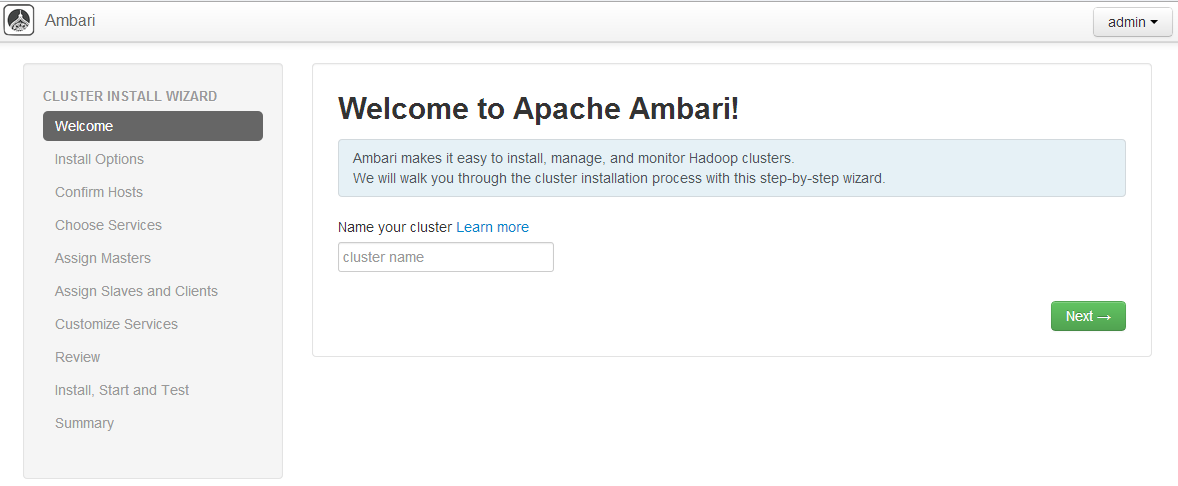
\includegraphics[width=.8\textwidth]{figs/5163os_06_14.png}
  \caption{Start Apache Ambari Installation}\label{fig:ambari.welcome}
\end{figure} 
Next, we need to configure the install options as shown in Figure \ref{fig:ambari.install.options}.
\begin{figure}[ht]
  \centering
  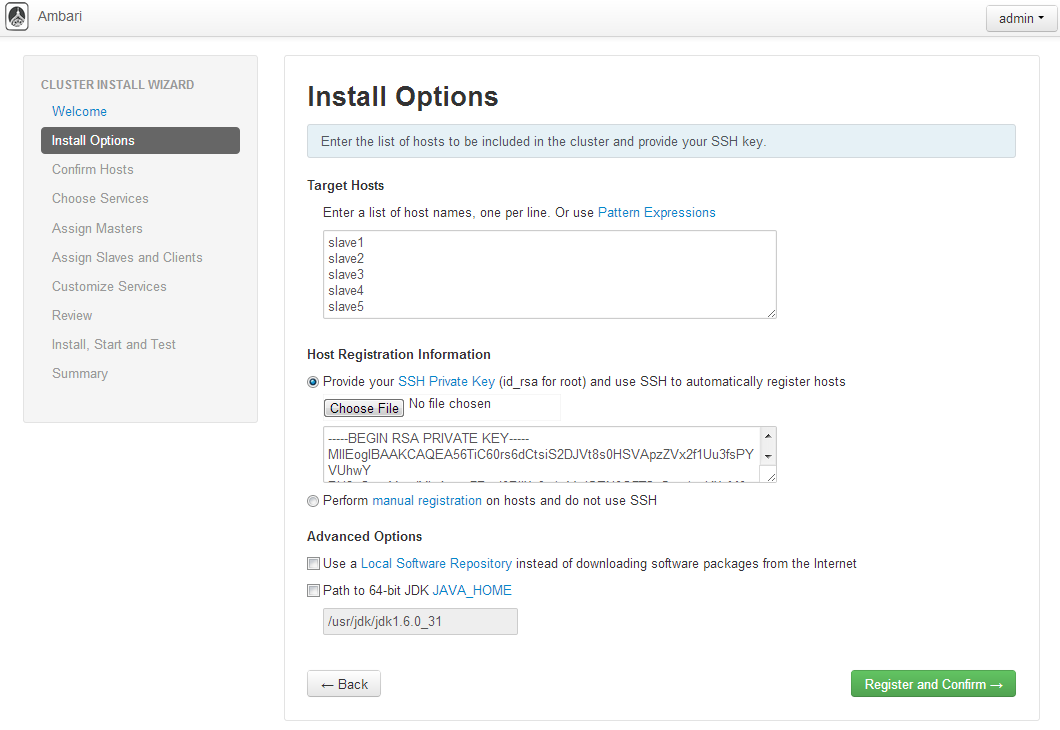
\includegraphics[width=.8\textwidth]{figs/5163os_06_15.png}
  \caption{Configure Installation Options}\label{fig:ambari.install.options}
\end{figure} 
After specifying the installation options as shown in Figure \ref{fig:ambari.install.options}, we can click the "Register and Confirm" button to start the installation process.  This will lead to the host registration progress page as shown in Figure \ref{fig:host.registration}. In this step, we need to confirm hosts to install Hadoop.
\begin{figure}[ht]
  \centering
  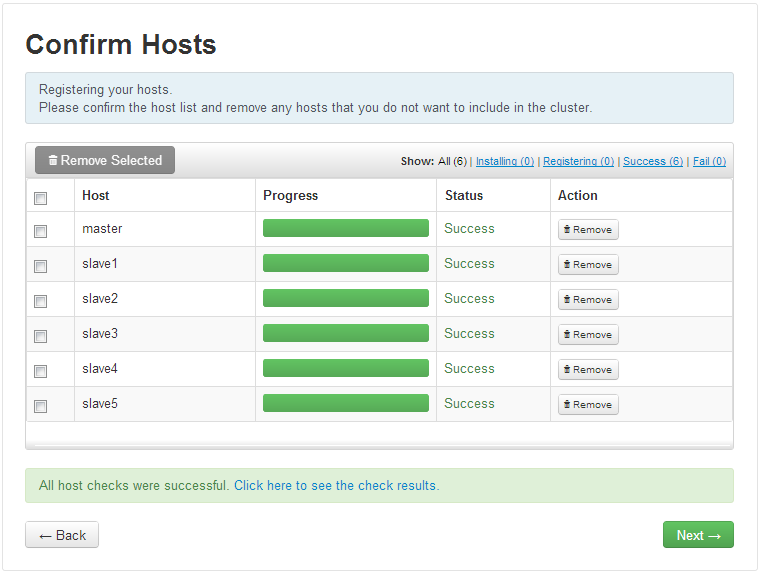
\includegraphics[width=.8\textwidth]{figs/5163os_06_17.png}
  \caption{Host Registration for the Hadoop Cluster}\label{fig:host.registration}
\end{figure} 
By clicking the "Next" button, we will go the a webpage to choose the services to install as shown in Figure \ref{fig:choose.services}.
\begin{figure}[ht]
  \centering
  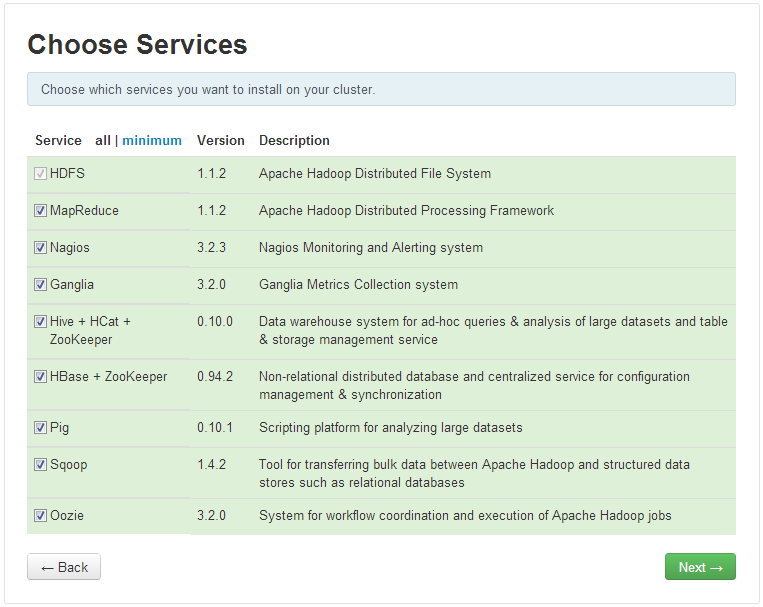
\includegraphics[width=.8\textwidth]{figs/5163os_06_18.png}
  \caption{Choose Services to Install}\label{fig:choose.services}
\end{figure} 
By default, all the services are selected to installed, we can make changes based on the requirements and then click the "Next" button. We will go to a webpage of to assign hosts as masters, slaves and clients, as shown in Figure \ref{fig:assign.masters}.
\begin{figure}[ht]
  \centering
  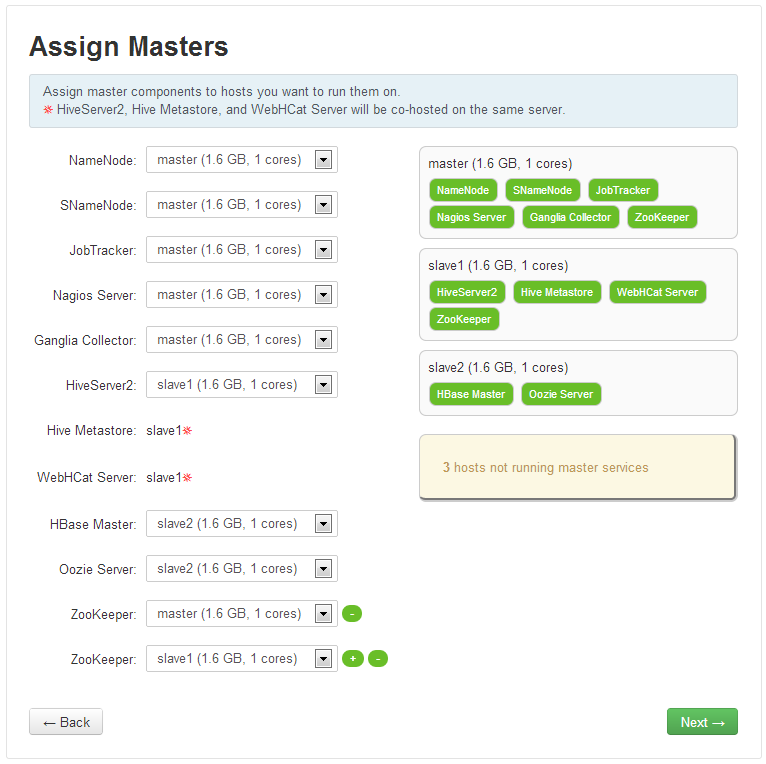
\includegraphics[width=.8\textwidth]{figs/5163os_06_19.png}
  \caption{Assign hosts for master nodes}\label{fig:assign.masters}
\end{figure} 

\begin{figure}[ht]
  \centering
  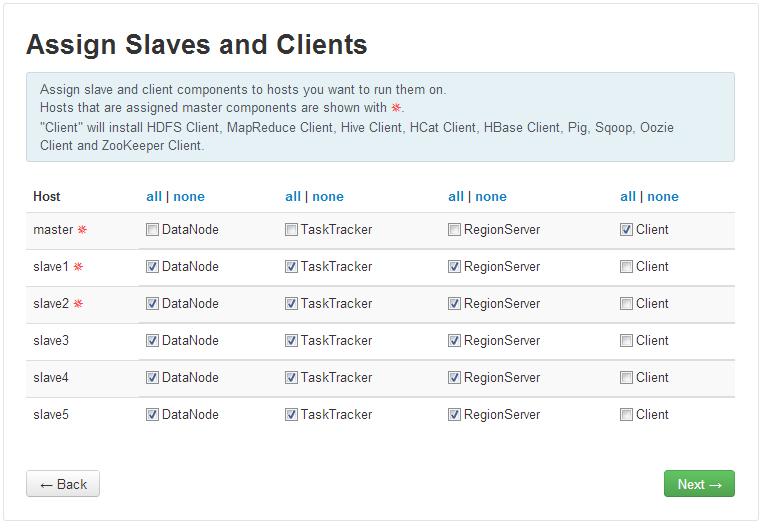
\includegraphics[width=.8\textwidth]{figs/5163os_06_20.png}
  \caption{Assign hosts for slaves and clients}\label{fig:assign.slaves}
\end{figure} 
Next, we will go to a webpage for customizing services, for example configuring the location for the NameNode directory. In this step, some services such as Hive and Nagios may ask you to enter administrative usernames and passwords, which are required for service installation.

After everything is configured, we will get a summary page about our configurations as shown in Figure \ref{fig:config.review}.
\begin{figure}[ht]
  \centering
  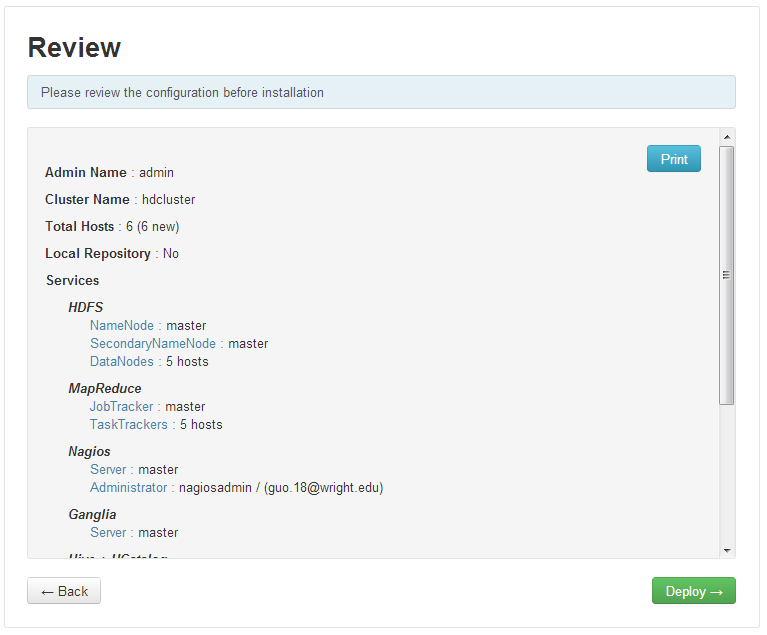
\includegraphics[width=.8\textwidth]{figs/5163os_06_22.png}
  \caption{Review Configuration before Installation}\label{fig:config.review}
\end{figure} 
By clicking on the "Deploy" button, the cluster deployment will start and a progress bar will appear for each service that is being installed as shown in Figure \ref{fig:hadoop.install.process}.
\begin{figure}[ht]
  \centering
  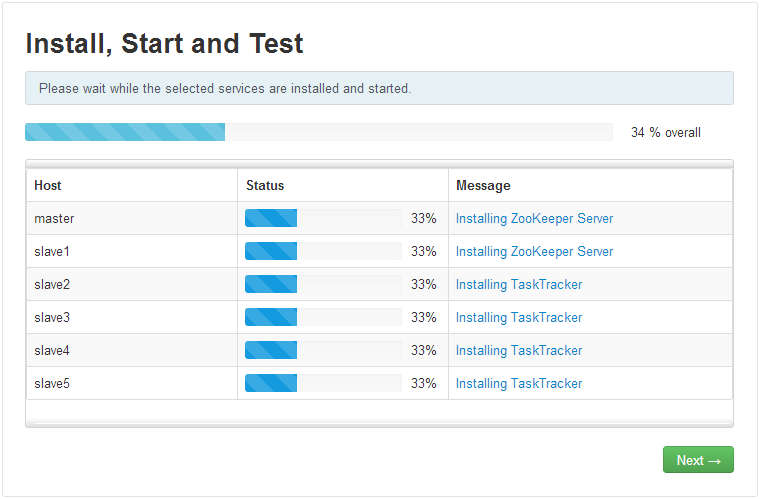
\includegraphics[width=.8\textwidth]{figs/5163os_06_24.png}
  \caption{The Hadoop Installation Process}\label{fig:hadoop.install.process}
\end{figure} 
After the deployment completes, we will get a summary page as shown in Figure \ref{fig:install.summary}.
\begin{figure}[ht]
  \centering
  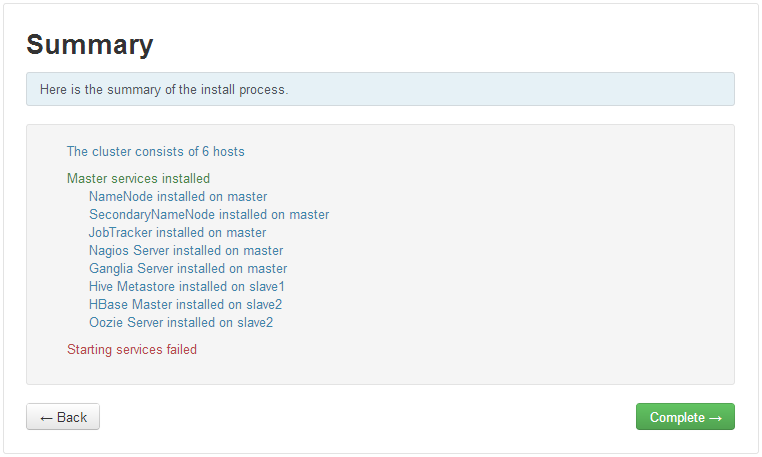
\includegraphics[width=.8\textwidth]{figs/5163os_06_26.png}
  \caption{Summary of the Installation Process}\label{fig:install.summary}
\end{figure} 
By clicking on the "Complete" button, the cluster installation process will complete, and we will be able to see the status of the cluster as shown in Figure \ref{fig:cluster.status}.
\begin{figure}[ht]
  \centering
  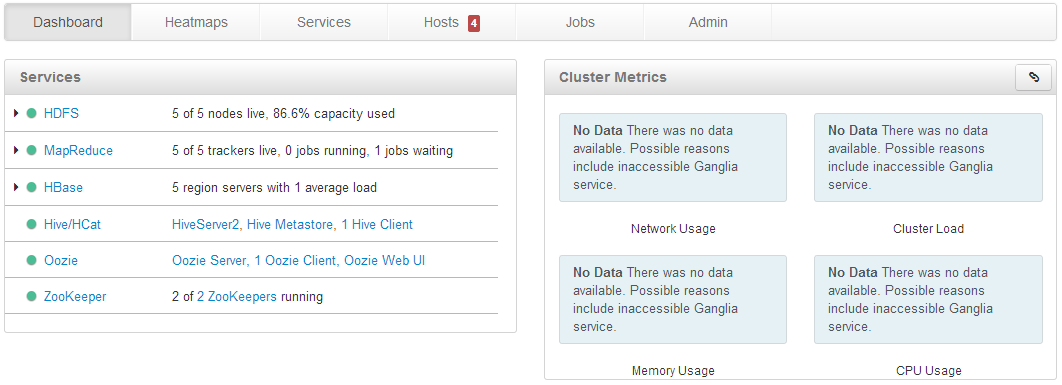
\includegraphics[width=.8\textwidth]{figs/5163os_06_27.png}
  \caption{Cluster Status after Installation}\label{fig:cluster.status}
\end{figure} 
\subsection*{See also}
\begin{itemize}
  \item Monitoring Hadoop cluster with JMX
  \item Monitoring Hadoop cluster with Chukwa 
  \item Monitoring Hadoop cluster with Ganglia
  \item Monitoring Hadoop cluster with Nagios
  \item \url{http://incubator.apache.org/ambari/}
  \item \url{http://incubator.apache.org/ambari/1.2.1/installing-hadoop-using-ambari/content/index.html}
\end{itemize}

\section{Monitoring Hadoop cluster with Chukwa}
Chukwa is a project developed for collecting and analysing Hadoop logs. It uses HDFS as its storage architecture and contains a number of toolkits for log analysis and cluster monitoring. In this recipe, we will guide you through steps to configure Chukwa to monitor a Hadoop cluster.
\subsection*{Getting ready}
Latest release of Chukwa uses HBase for key-value storage. So, before getting started, we assume that Hadoop and HBase have been installed and properly configured.

Next, we can use the following steps to install Chukwa:

Download the latest release from the official website \url{http://incubator.apache.org/chukwa}, for example, use command:
\lstset{style=bashstyle}
\begin{lstlisting}[language=bash]
$ sudo wget http://mirror.symnds.com/software/Apache/incubator/chukwa/chukwa-0.5.0/chukwa-incubating-src-0.5.0.tar.gz -P /usr/local
\end{lstlisting}

Decompress the archive with command: \\
\verb|$ sudo tar xvf chukwa-incubating-src-0.5.0.tar.gz|

Create symbolic link from for the directory with: \\
\verb|$ sudo ln -s chukwa-incubating-src-0.5.0 chukwa|

Change ownership for the directories with: 
\lstset{style=bashstyle}
\begin{lstlisting}[language=bash]
$ sudo chown hduser.hduser chukwa-incubating-src-0.5.0 -R
$ sudo chown hduser.hduser chukwa -R
\end{lstlisting}

Change environment variables by adding the following content into the \verb|~/.bashrc| file: 
\lstset{style=bashstyle}
\begin{lstlisting}
export CHUKWA_HOME=/usr/local/chukwa
PATH=$CHUKWA_HOME/bin:$PATH
\end{lstlisting}

Build Chukwa from source with command: 
\lstset{style=bashstyle}
\begin{lstlisting}[language=bash]
$ source ~/.bashrc
$ cd $CHUKWA_HOME
$ mvn clean package
\end{lstlisting}

When compile finishes, the directory structure of Chukwa will be similar to the following:\\
\verb|$ chukwa|

%% [TODO add content here. ]

If you are downloading the binary version of Chukwa, the directory structure might be different from this.

Install telnet with command: \\
\verb|$ sudo yum install telnet| \\

Login to the master node from administrator machine with command: \\
\verb|$ ssh hduser@master|

\subsection*{How to do it...}
Use the following recipe to configure Chukwa for Hadoop monitoring:

Change the \verb|log4j.appender.DRFA| variable in file \verb|$HADOOP_HOME/conf/log4j.properties| to be the following: \\
\verb|log4j.appender.DRFA=org.apache.log4j.net.SocketAppender|

Copy the Hadoop metrics file from the Chukwa directory to the Hadoop configuration directory with:
\lstset{style=bashstyle}
\begin{lstlisting}[language=bash]
$ cp $CHUKWA_HOME/etc/chukwa/hadoop-metrics.properties $HADOOP_HOME/conf
\end{lstlisting}

Copy the client jar file from the Chukwa installation directory to the Hadoop shared directory with:
\lstset{style=bashstyle}
\begin{lstlisting}[language=bash]
$ cp $CHUKWA_HOME/share/chukwa/chukwa-0.5.0-client.jar $HADOOP_HOME/lib
\end{lstlisting}

Copy the json library from the Chukwa library to the Hadoop library with:
\lstset{style=bashstyle}
\begin{lstlisting}[language=bash]
$ cp $CHUKWA_HOME/share/chukwa/lib/json-simple-1.1.jar $HADOOP_HOME/lib
\end{lstlisting}

Sync the files and configurations to the slave nodes with command: 
\lstset{style=bashstyle}
\begin{lstlisting}[language=bash]
for host in `cat $HADOOP_HOME/conf/slaves`
do
  echo "Copying file to " $host
  scp $HADOOP_HOME/lib/chukwa-0.5.0-client.jar $host:$HADOOP_HOME/lib;
  scp $HADOOP_HOME/lib/json-simple-1.1.jar $host: $HADOOP_HOME/lib;
  scp $HADOOP_HOME/conf/hadoop-metrics.properties $host:$HADOOP_HOME/conf
done
\end{lstlisting}

Restart the Hadoop cluster with command: \\
\verb|$ stop-all.sh| \\
\verb|$ start-all.sh|

Start the HBase daemon with command: \\
\verb|$ start-hbase.sh|

Import the Chukwa schema file to HBase with:
\lstset{style=bashstyle}
\begin{lstlisting}
$ hbase shell < $CHUKWA_HOME/etc/chukwa/hbase.schema
HBase Shell; enter 'help<RETURN>' for list of supported commands.
Type "exit<RETURN>" to leave the HBase Shell
Version 0.94.5, r1443843, Fri Feb  8 05:51:25 UTC 2013

create "Hadoop",
{NAME => "ClientTrace", VERSIONS => 65535},
{NAME => "dfs_namenode", VERSIONS => 65535},
{NAME => "dfs_FSNamesystem", VERSIONS => 65535},
{NAME => "dfs_datanode", VERSIONS => 65535},
{NAME => "mapred_jobtracker", VERSIONS => 65535},
{NAME => "mapred_shuffleOutput", VERSIONS => 65535},
{NAME => "mapred_tasktracker", VERSIONS => 65535},
{NAME => "jvm_metrics", VERSIONS => 65535},
{NAME => "mapred_Queue", VERSIONS => 65535},
{NAME => "metricssystem_MetricsSystem", VERSIONS => 65535},
{NAME => "rpc_rpc", VERSIONS => 65535},
{NAME => "rpcdetailed_rpcdetailed", VERSIONS => 65535},
{NAME => "ugi_ugi", VERSIONS => 65535}
0 row(s) in 2.7920 seconds

create "HadoopLog",
{NAME => "NameNode", VERSIONS => 65535},
{NAME => "Audit", VERSIONS => 65535}
0 row(s) in 1.0740 seconds

create "Jobs",
{NAME => "summary" }
0 row(s) in 1.0610 seconds

create "SystemMetrics",
{NAME => "cpu", VERSIONS => 65535},
{NAME => "system", VERSION => 65535},
{NAME => "disk", VERSION => 65535},
{NAME => "memory", VERSION => 65535},
{NAME => "network", VERSION => 65535},
{NAME => "tags", VERSION => 65535}
0 row(s) in 1.1030 seconds

create "ClusterSummary",
{NAME=> "cpu", VERSIONS => 65535},
{NAME => "system", VERSION => 65535},
{NAME => "disk", VERSION => 65535},
{NAME => "memory", VERSION => 65535},
{NAME => "network", VERSION => 65535},
{NAME => "hdfs", VERSION => 65535},
{NAME => "mapreduce", VERSION => 65535}
0 row(s) in 1.0830 seconds

create "chukwa",
{NAME=>"chukwaAgent_chunkQueue", VERSIONS => 65535},
{NAME => "chukwaAgent_metrics", VERSION => 65535},
{NAME => "chukwaAgent_httpSender", VERSION => 65535}
0 row(s) in 1.0860 seconds
\end{lstlisting}

The output shows that six HBase tables have been created.

Use a text editor to open file \verb|$CHUKWA_HOME/etc/chukwa/chukwa-collector-conf.xml| and comment the chukwaCollector.pipeline property by adding the following strings before and after the property: \\
\verb|<!--|\\
and

\verb|-->|

By doing this, we have configured Chukwa to use HBase for log collection storage.

Configure the environment variables in file \verb|$CHUKWA_HOME/etc/chukwa/chukwa-env.sh| to the following: 
\lstset{style=bashstyle}
\begin{lstlisting}
export JAVA_HOME=/usr/java/latest
export HADOOP_HOME=/usr/local/hadoop
export HBASE_HOME=/usr/local/hbase
export HADOOP_CONF_DIR=$HADOOP_HOME/conf
export HBASE_CONF_DIR=$HBASE_HOME/conf
\end{lstlisting}

Configure Chukwa to collect data from slave nodes by adding the following hostnames to file \verb|$CHUKWA_HOME/etc/chukwa/agents|: 
\begin{verbatim}
slave1
slave2
slave3
...
\end{verbatim}

We can run multiple collectors (for example, we want to run collectors on master node and the slave1 node) by adding the following content into file \verb|$CHUKWA_HOME/etc/chukwa/collectors|: 
\begin{verbatim}
http://master:8081
http://slave1:8081
\end{verbatim}

Multiple collectors can increase the throughput of the data collection process.

Start Chukwa agents with command: 
\lstset{style=bashstyle,language=bash}
\begin{lstlisting}
$ start-agents.sh
slave4: starting agent, logging to /tmp/chukwa/logs/chukwa-hduser-agent-slave4.out
slave5: starting agent, logging to /tmp/chukwa/logs/chukwa-hduser-agent-slave5.out
slave1: starting agent, logging to /tmp/chukwa/logs/chukwa-hduser-agent-slave1.out
slave3: starting agent, logging to /tmp/chukwa/logs/chukwa-hduser-agent-slave3.out
slave2: starting agent, logging to /tmp/chukwa/logs/chukwa-hduser-agent-slave2.out
\end{lstlisting}

Start Chukwa collector with command: 
\lstset{style=bashstyle}
\begin{lstlisting}
$ start-collectors.sh
master: starting collector, logging to /tmp/chukwa/logs/chukwa-hduser-collector-master.out
slave1: starting collector, logging to /tmp/chukwa/logs/chukwa-hduser-collector-slave1.out
\end{lstlisting}

Add configuration directory of Hadoop and HBase to Pig CLASSPATH with: \\
\verb|export PIG_CLASSPATH=$HADOOP_HOME/conf:$HBASE_HOME/conf|

Use pig to analyze the data with command:
\lstset{style=bashstyle}
\begin{lstlisting}[language=bash]
$ pig -Dpig.additional.jars=$HBASE_HOME/hbase-0.94.5.jar:$PIG_HOME/pig-0.11.0.jar $CHUKWA_HOME/share/chukwa/script/pig/ClusterSummary.pig
\end{lstlisting}

Start the web UI for Hadoop Infrastructure Care Center (HICC) with command: \\
\verb|$ chukwa hicc|

Open URL: \url{http://master:4080} and use admin as both user name and password for login.

We can modify file \verb|$CHUKWA_HOME/etc/chukwa/auth.conf| to change the login credential.

By default the file will have the following content:\\
\verb|admin: admin, user|

The meaning of this is username: \verb|password[, role]|

\subsection*{How it works}
Chukwa was designed to collect data that are dynamically generated across distributed machines in a cluster. It has four major components: adaptor, collector, MapReduce or other data processing jobs and the web UI called HICC.

Chukwa adaptors are deployed on each data source machines. Adaptors run on these machines in the umbrella of agents, which send the collected data to collectors on local or remote machines.

Chukwa collectors pipeline data from agents to data storage systems such as HDFS. For performance reasons, data are typically written as sequence files, which will be processed by MapReduce jobs.

The MapReduce jobs will generate key-value pairs for visualization by the last component HICC. Chukwa uses the embedded web server Jetty for the deployment of the web archive file \verb|$CHUKWA_HOME/ share/chukwa/webapps/hicc.war|.

Sometimes, you might have problem running the HICC and visiting web UI, the most probable reason is that you have incompatible jar files for Hadoop, HBase and Chukwa. In such cases, my suggestion is to clone the source code from \href{https://github.com/apache/chukwa}{github} and compile the hicc.war web archive file from source. For more information, please check the \verb|README.txt| file in the source code root directory.

In summary, the data flow of Chukwa can be described with the following figure:
\begin{figure}[ht]
  \centering
  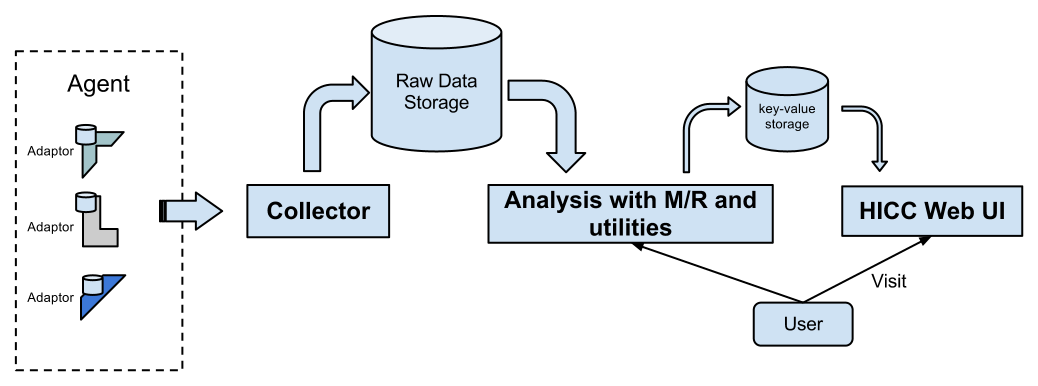
\includegraphics[width=\textwidth]{figs/5163os_06_08.png}
  \caption{Chukwa Dataflow}\label{fig:chukwa.dataflow}
\end{figure} 
For more information about the design of Chukwa, please check the \href{http://incubator.apache.org/chukwa/docs/r0.5.0/design.html}{documentation}.

\subsection*{There's more...}
Due to the instability of this software package, you might need to do some debugging when deploying it onto the cluster. But to get started with Chukwa, it is always advisable to run in local or pseudo-distributed mode, which will start one agent and one collector on the local machine. To do this, the following commands can be used:
\lstset{style=bashstyle}
\begin{lstlisting}
$ chukwa agent local
OK chukwaAgent.checkpoint.dir [File] = /tmp/chukwa/log/
OK chukwaAgent.checkpoint.interval [Time] = 5000
OK chukwaAgent.control.port [Portno] = 9093
OK chukwaAgent.sender.fastRetries [Integral] = 4

chukwa collector local
OK chukwaCollector.http.port [Integral] = 8081
OK chukwaCollector.pipeline [ClassName list] = org.apache.hadoop.chukwa.datacollection.writer.SocketTeeWriter,org.apache.hadoop.chukwa.datacollection.writer.hbase.HBaseWriter
OK chukwaCollector.rotateInterval [Time] = 300000
OK chukwaCollector.writerClass [ClassName] = org.apache.hadoop.chukwa.datacollection.writer.PipelineStageWriter
OK writer.hdfs.filesystem [URI] = hdfs://master:54310
started Chukwa http collector on port 8081
\end{lstlisting}

We can check the status of the daemons by tailing on the log files with the following commands:
\verb|$ tail -f /tmp/chukwa/logs/agent.log| \\
\verb|$ tail -f /tmp/chukwa/logs/collector.log|

Currently, Chukwa is an incubator project under Apache Free Software (AFS) foundation. We can check the development plan and progress on its wiki page wiki.apache.org/hadoop/chukwa or on \href{http://incubator.apache.org/chukwa/}{the official site}. Similar to many open source projects, new bugs are reported and new features added, a nice way to keep up to date with the most recent changes is to work with the source \href{https://github.com/apache/chukwa}{code repository}.
\subsection*{See also}
\begin{itemize}
  \item Monitoring Hadoop cluster with JMX
  \item Monitoring Hadoop cluster with Ganglia
  \item Monitoring Hadoop cluster with Nagios
  \item Monitoring Hadoop cluster with Ambari
  \item \url{http://incubator.apache.org/chukwa/docs/r0.5.0/admin.html}
\end{itemize}
